\documentclass[10pt,norsk,a4paper]{article}
\usepackage[utf8]{inputenc}
\usepackage[T1]{fontenc}
\usepackage[norsk]{babel}
% - PDF-relatert
\usepackage{hyperref,pdfpages,hypcap}
\hypersetup{colorlinks=true,allcolors=.}
\newcommand\fhref[2]{%
	\href{#1}{#2}\footnote{\url{#1}}%
}
% Andre pakker
\usepackage[cm]{fullpage}
\usepackage{parskip,multicol,textcomp,amssymb,graphicx,color,enumitem,cleveref}
% - Korreksjon av fotnoter i seksjoner/overskrifter
\usepackage[stable]{footmisc}
% - Skrifttype
\usepackage[bitstream-charter]{mathdesign}
% - Kommentarer
\usepackage{comment}
\usepackage{epstopdf}

\epstopdfsetup{outdir=./}


\title{Generalforsamling \\
	Høsten 2020\\[3cm]
	
\includegraphics[width=0.5\textwidth]{cyb-logo.eps}\\[-.5cm]}
\date{26.\ november 2020}
\author{Cybernetisk Selskab}

% Blank header, samt footer med side x av y
\usepackage{fancyhdr}
\pagestyle{fancy}
\renewcommand{\headrulewidth}{0pt}
\fancyhead{}
\cfoot{Side~\thepage\ av~\pageref*{lastpage}}


\begin{document}

\maketitle{}
\newpage
\tableofcontents

\section{Valg av møteleder}

\section{Valg av referent}

\section{Valg av protokollunderskrivere}

\section{Valg av tellekorps}

\section{Godkjenning av innkalling}

\section{Godkjenning av dagsorden}

\section{Semesterberetninger}
\subsection{Semesterberetning ved leder}

Kjære interne, medlemmer og andre studenter.

\begin{multicols}{2}
Takk for at dere alle har dukket opp på denne digitale 
generalforsamlingen, til tross for at det er den andre 
på kort tid. Dette blir av den grunn en ganske kort 
semesterberetning, hvis man i det hele tatt kan kalle 
to måneder et semester.\\
Siden sist har vi hatt en god periode med mye aktivitet 
og god steming til tross for omstendighetene, dessvere 
måtte vi jo stenge ned det meste av aktivitet igjen 
ettersom situasjonen i Oslo forverret seg, men vi 
forsøker å holde det gående digitalt. Det har vært godt 
oppmøte på de digitale kosetirsdagene og digital quiz, 
dette er oppmuntrende!\\
Vi har fått inn flere nye interne, og de nye 
styremedlemmene har de siste to månedene tredd in i rollen 
sin på en god måte. Dette har bidratt til å lette litt 
på lasten til oss som har sittet en stund, jeg håper vi 
kan få inn enda flere nye i dag slik at vi kan fortsette 
å bevege oss i en retning hvor det ikke er alt for mye 
arbeid på noen få.\\

Takk til alle de frivillige som gjør CYB mulig!\\
\end{multicols}

\textbf{Martin Heggem}, \\
leder, \date{\emph{26. november 2020}}

\subsection{Semesterberetning ved kjellermogul}

\begin{multicols}{2}
Dette semesteret har vi vært heldige med å kunne være åpne 
lenge. Store smittetall til tross. Intrykket jeg har fått 
gjennom semesteret er at studenter, og spesielt våre frivillige 
har tatt dette på alvor. Dette har de til tross, tidvis 
dårlig informasjon og korte frister. Fristene til Oslo komune 
har tidvis ført til forvirring hos oss, ettersom de har medført 
at vi må omstille oss på relativt kort tid.\\
Det har også vært mye godt engasjement og overraskende mange 
nye frivillige, til tross for pandemien. Dette tror jeg har 
sågar som kommer til å styrke og forbedre miljøet i foreningen. 
Disse nye frivillige har vist godt initiativ og en vilje til 
å bidra til fellesmiljøet gang på gang. \\ 
Blandt besølkende har vi hatt stor pågang tiltross for redusert 
kapasitet. Det har også vært veldig mye positivitet rundt 
bordservering hos oss. Våre besøkende har vært lydhør 
irettesettelse og vært positive, situasjonen til tross. Dette 
er noe jeg tror gjør det enda hyggeligere å jobbe i bar.\\
Vi har også fått system med edru ansvarlig på internarrangement. 
Dette gjør at internarrangement ikke er like gråsone lengere 
og vi har mye bedre kontroll og oversikt på disse arangementene. 
Jeg vil gjerne nevne at de som har stått under de få internfestene 
vi har hatt, har gjort en super jobb. \\
Vi ikke altid like flinke til å si dette i foreningen, men alle 
frivillige har vist en ufattelig ståpåvilje dette semesteret. 
Dere har vært hyggelige og en sann fryd å ha med å gjøre. Ser 
frem til å tilbringe flere semestere med dere.\\

\end{multicols}
\textbf{Boye Mathias Moltegerg}, \\
kjellermogul, \date{\emph{26. november 2020}}

\section{Regnskap}
Økonomiansvarlig orienterer foreningen om status for regnskapene.

\section{Budsjett}
Økonomiansvarlig redegjør for budsjett 2021.

\section{Kontingentfastsettelse}
Hovedstyret foreslår å beholde kontingenten på 50 kr per semester.

\section{Valg}
\subsection{Hovedstyret}
Man velges inn i hovedstyret for ett år av gangen. Vervene leder, 
nestleder, arrangementssjef og internansvarlig er ikke på valg. 
I dag har Martin Heggem, Olav Aga, Jørgen Spilling og Jakob 
Gundersen disse vervene.

\begin{multicols}{2}
\subsubsection{Kasserer}
\textbf{Kasserer} leder økonomigruppa og har ansvaret for økonomien i foreningen, herunder
budsjett og regnskap.
\\\\\textit{Kasserer presenterer vervet.}

\subsubsection{Kjellermogul}
\textbf{Kjellermogul} er leder av Kjellerstyret og daglig leder i
Escape. Og har dermed det overordnede ansvaret for alt som foregår på
Escape.
\\\\\textit{Kjellermogul presenterer vervet.}

\subsubsection{Promoteringssjef}
\textbf{Promoteringssjef} leder promoteringsgruppen som har ansvar for å
utarbeide grafisk materiell til arrangementene i foreningen og skape
blest rundt disse.
\\\\\textit{Promoteringssjef presenterer vervet.}

\subsubsection{Rekrutteringsansvarlig}
\textbf{Rekrutteringsansvarlig} har som ansvar å få inn nye frivillige i
CYB. Rekrutteringsansvarlig setter potensielle interne i kontakt med
gruppeledere.
\\\\\textit{Rekrutteringsansvarlig presenterer vervet.}

\end{multicols}

\newpage
\subsection{Kjellerstyret} 
Alle verv som er til valg i kjellerstyret gjelder for ett semester av 
gangen. Med unntak av Økonomiansvarlig som blir valgt inn for to semester.
Kjellermogul sitter også i kjellerstyret i tillegg til hovedstyret. 

\begin{multicols}{2}

\subsubsection{Kjellernestleder}

\textbf{Kjellernestleder} er nestleder i kjellerstyret, og gjør bidrar
med ulike oppgaver ved behov. Nestleder er også kjellermoguls venstre
hånd og stedfortreder, og skal kunne tre inn om kjellermogul skulle være
utilgjengelig.\\\\
\textit{Kjellernestleder presenterer vervet.}

\subsubsection{Økonomiansvarlig}
\textbf{Økonomiansvarlig} jobber tett med kasserer og har ansvaret for
den daglige økonomidriften av Escape.\\\\
\textit{Økonomiansvarlig presenterer vervet.}

\subsubsection{Barsjef}
\textbf{Barsjef} er nestleder i Kjellerstyret, og er derfor
ansvarsperson etter Kjellermogul. Hovedansvaret ligger i drift av bar. \\\\
\textit{Kjellermogul presenterer vervet.}

\subsubsection{Kafésjef}
\textbf{Kafésjef} er ansvarlig for å drive kaféen på dagtid i Escape og
har tett kontakt og oppfølgning av de frivillige i kaféen.
\\\\\textit{Kafésjef presenterer vervet.}

\subsubsection{Innkjøpsansvarlig}
\textbf{Innkjøpsansvarlig} har ansvar for å kjøpe inn det som trengs til
driften av Escape.
\\\\\textit{Innkjøpsansvarlig presenterer vervet.}

\subsubsection{Teknisk sjef}
\textbf{Teknisk} sjef er en altmuligmann(-kvinne) som sørger for at alt
teknisk utstyr i Escape fungerer i tilfredsstillende grad.
\\\\\textit{Teknisk sjef presenterer vervet.}

\subsubsection{Utlånsansvarlig}
\textbf{Utlånsansvarlig} organiserer utlån av Escape, og pleier også å
være CYBs representant i Studentkjellernes personalforening.
\\\\\textit{Utlånsansvarlig presenterer vervet.}

\subsubsection{DJ-sjef}
\textbf{DJ-sjef} har ansvar for opplæring, rekruttering og mobilisering
av DJ-er til kveldsarrangementer, samt håndheve musikkprofil og skape
god stemning.
\\\\\textit{DJ-sjef presenterer vervet.}

\subsubsection{Arrangementskoordinator}
\textbf{Arrangementskoordinator} er bindeledd mellom bargruppa,
arrangementsgruppa og kjellerstyret for arrangementer med hovedvekt på
spritbardrift.
\\\\\textit{Arrangementskoordinator presenterer vervet.}
\end{multicols}

\section{Vedtektsforslag}
Det har ikke kommet inn noen endringsforslag til vedtektene innen fristen.

\part*{Vedlegg}\label{lastpage}
\addcontentsline{toc}{part}{Vedlegg}

\phantomsection{}
\addcontentsline{toc}{section}{Vedtekter for Cybernetisk Selskab} % chktex
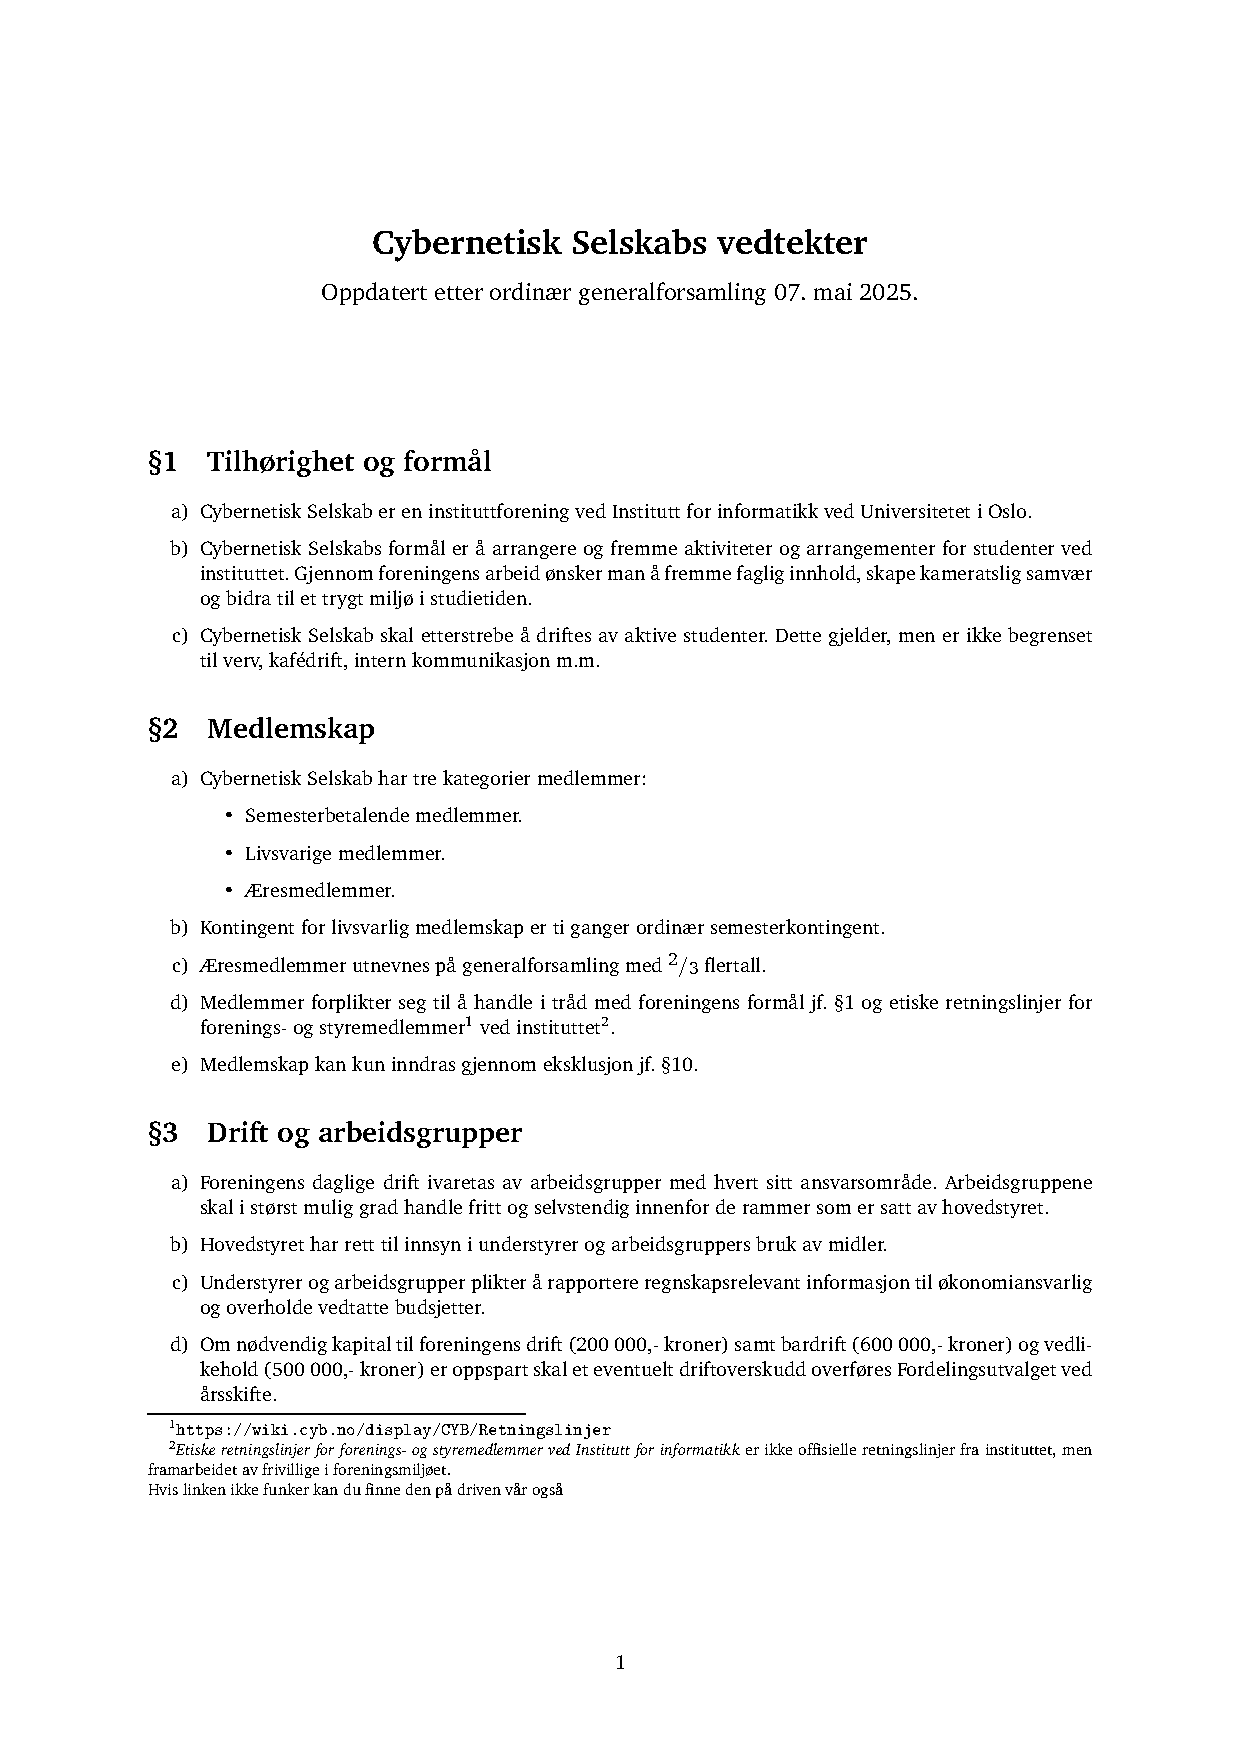
\includepdf[pages=-]{../vedtekter/vedtekter.pdf}

\end{document}
